\documentclass{article}
\usepackage[T1]{fontenc}
\usepackage[portuguese]{babel}
%\usepackage[htt]{hyphenat}
\usepackage{times}
\usepackage{color}
\usepackage{anppom2008}

\newcounter{notecounter}

\newcommand{\note}[1]{
  \addtocounter{notecounter}{1}
  \textcolor{red}{[note \arabic{notecounter}: #1]}
}

\newcommand{\rameau}{\textit{Rameau}}

\begin{document}
\graphicspath{{figs/}}

\title{Título do trabalho}
\author{Autor}{Filiação acadêmica}{e-mail}{website}

\begin{sumario}
  Resumo do texto com até 100 palavras.  
\end{sumario}

\keywords{até cinco palavras-chave que descrevam o assunto do texto}

\section{Introdução}
\label{sec:introducao}


\section{Rameau}
\label{sec:rameau}

Todo o trabalho descrito nesse artigo foi desenvolvido usando o
sistema \rameau{} \note{citar icmc? kroger: sim} para análise
automática de harmonia e extração de informação musical. \rameau{} é
um framework para implementação de algoritmos de análise harmônica de
partituras simbólicas. As partituras são guardadas em arquivos no
formato Lilypond \cite{nienhuys.ea08:lilypond}, que permite
diferenciação de notas enarmônicas e geração de partituras bem
tipografadas. As notas são extraídas das partituras e apresentadas a
uma rede neural, que associa cada conjunto de notas a um acorde. Para
esse trabalho, o \rameau{} foi extendido para realizar operações
comuns de musicologia, como detecção de cruzamentos, quintas ou
oitavas consecutivas, cadências frequentes, etc.

Além disso \rameau{}  possui vários outros algoritmos para análise
harmônica, como o de Pardo e Birmingham \cite{pardo.ea00:automated},
outras redes neurais e classificadores de árvores de decisão e
k-vizinhos-mais-próximos. Atualmente \rameau{}  está sendo extendido para
realizar análise funcional de qualquer peça tonal.

\section{Análise}
\label{sec:analise}

\subsection{Âmbitos}
\label{sec:ambitos}


* soprano

graves

186 034* 050 068 075 223 049 070 100 165 185 197 214 325 348 158 175
205 239 352 087 110 244

agudos

116 254 282 298 331 334

* alto

graves

345 186

agudos

024 028 033 036 057 058 069 078 084 123 217 225 248 252 329 331 334
354 359

* tenor

graves

229 070 205

agudos

024 043 074 083 151 156 224 248 263 264 273 276 281 329 354 371

* baixo

graves

034 051 214 223 340 131 328 143 155 197 205 219 241 187 235 319 337
240 070 075 165 175 239

agudos

285 312 331

\begin{figure}
  \centering
  \includegraphics[scale=2.5]{ambitos}
  \caption{Comparação de âmbito utilizado por Bach e definido por
    Kostka e Payne}
  \label{fig:ambito-kostka}
\end{figure}

\subsection{Cruzamento de vozes}
\label{sec:cruzamento-de-vozes}

851 cruzamentos 

para evitar quintas e oitavas consecutivas

para manter melhor condução de vozes

\subsection{Quintas e oitavas consecutivas}
\label{sec:quintas-e-oitavas}

fermata (continuação)

sem razao 118, 152, 244, 279 (oitava-unissono), 239

nota melodica 351

\begin{figure}
  \centering
  \subfigure[Coral 244]{
    \includegraphics[scale=5]{244-oitava}
  }
  \qquad
  \subfigure[Coral 279]{
    \includegraphics[scale=2.7]{279-oitava}
  }
  \qquad
  \subfigure[Coral 329]{
    \includegraphics[scale=2.8]{329-oitava}
  }
  \caption{Oitavas e uníssonos}
  \label{fig:oitavas-e-unissonos}
\end{figure}

\subsection{Sétimas}
\label{sec:setimas}

acorde de passagem

bizarro

arpejo

perde sétima

ascendente

(ver setimas koechlin)

\begin{figure}
  \centering
  \subfigure[Ascendente cromática]{
    \includegraphics[scale=3]{003-setima-asc-crom}
  }
  \subfigure[Vozes de passagem]{
    \includegraphics[scale=5]{015-setima-acorde-pass}
  }
  \subfigure[Arpejo antes da resolução]{
    \includegraphics[scale=3]{049-setima-arpejo}
  }
  \subfigure[Sétima transformada em nota do acorde seguinte]{
    \includegraphics[scale=5]{120-setima-koechlin}
  }
  \caption{Resoluções de sétima}
  \label{fig:setima-resol}
\end{figure}

\renewcommand{\refname}{Referências Bibliográficas}
\bibliographystyle{kchicago}
\bibliography{writing-style,harmonic-analysis,melodic-contour,music-harmony-and-theory,programs}

\end{document}
